\documentclass[utf8]{beamer}

\mode<presentation>
{
  \usetheme{Warsaw}
  \setbeamercovered{transparent}
}


\usepackage{amsfonts,mathtools,amssymb}
\usepackage[spanish]{babel}
\usepackage{times}
\usepackage[T1]{fontenc}
\usepackage[shortlabels]{enumitem}
\usepackage{tikz}
\usepackage{physics}

\title[MA0505]{MA0505 - An\'alisis I}
\subtitle{Lecci\'on XII: La Medida Exterior}

\author{Pedro M\'endez\inst{1}}

\institute[Universidad de Costa Rica] % (optional, but mostly needed)
{
  \inst{1}%
  Departmento de Matem\'atica Pura y Ciencias Actuariales\\
  Universidad de Costa Rica
  }

\date[I-2021] {Semestre I, 2021}

%%%%%%%%% === Theorems and suchlike === %%%%%%%%%%%%%%

\theoremstyle{plain}
\newtheorem{Th}{Teorema}               %%% Theorem 1.1.1
\newtheorem{Tmon}{Teoremón}
\newtheorem{Prop}{Proposición}         %%% Proposition 1.1.2
\newtheorem{Lem}{Lema}                 %%% Lemma 3
\newtheorem{Cor}{Corolario}            %%% Corollary 4

\theoremstyle{definition}
\newtheorem{Def}{Definición}           %%% Definition 5
\newtheorem{Ex}{Ejemplo}               %%% Example 6
\newtheorem{Ej}{Ejercicio}             %%% Ejercicio 7
\newtheorem{Hec}[Th]{Hecho}            %%% Hecho 1.1.8

\theoremstyle{remark}
\newtheorem{Rmk}[Th]{Observación}      %%%Remark 1.1.9
\newtheorem*{nonum-Rmk}{Observación}         %%% No number Fact
\newtheorem*{Notn}{Notaci\'on}        %% Notaciones
\newtheorem*{Warn}{Advertencia}       %% Advertencias

\numberwithin{equation}{section}

%% Accomodations 

\makeatletter
\def\moverlay{\mathpalette\mov@rlay}
\def\mov@rlay#1#2{\leavevmode\vtop{%
   \baselineskip\z@skip \lineskiplimit-\maxdimen
   \ialign{\hfil$\m@th#1##$\hfil\cr#2\crcr}}}
\newcommand{\charfusion}[3][\mathord]{
    #1{\ifx#1\mathop\vphantom{#2}\fi
        \mathpalette\mov@rlay{#2\cr#3}
      }
    \ifx#1\mathop\expandafter\displaylimits\fi}
\makeatother

% Greek letters:

\newcommand{\al}{\alpha}                %% short for  \alpha
\newcommand{\bt}{\beta}                 %% short for  \beta
\newcommand{\Dl}{\Delta}                %% short for  \Delta
\newcommand{\dl}{\delta}                %% short for  \delta
\newcommand{\eps}{\varepsilon}          %% short for  \varepsilon
\newcommand{\Ga}{\Gamma}                %% short for  \Gamma
\newcommand{\ga}{\gamma}                %% short for  \gamma
\newcommand{\La}{\Lambda}               %% short for  \Lambda
\newcommand{\la}{\lambda}               %% short for  \lambda
\newcommand{\Om}{\Omega}                %% short for  \Omega
\newcommand{\om}{\omega}                %% short for  \omega
\newcommand{\Sg}{\Sigma}                %% short for  \Sigma
\newcommand{\sg}{\sigma}                %% short for  \sigma
\newcommand{\te}{\theta}                %% short for  \theta
\newcommand{\vf}{\varphi}               %% short for  \varphi
\newcommand{\ze}{\zeta}                 %% short for  \zeta

%Boldface letters

\newcommand{\bC}{\mathbb{C}}    %%% números complejos
\newcommand{\bN}{\mathbb{N}}    %%% números naturales
\newcommand{\bP}{\mathbb{P}}        %% números enteros positivos
\newcommand{\bQ}{\mathbb{Q}}    %%% números racionales
\newcommand{\bR}{\mathbb{R}}    %%% números reales
\newcommand{\bS}{\mathbb{S}}    %%% esfera
\newcommand{\bZ}{\mathbb{Z}}    %%% números enteros

%Script letters:

\newcommand{\cA}{\mathcal{A}}           %% formas diferenciales
\newcommand{\cB}{\mathcal{B}}           %% una base vectorial
\newcommand{\cC}{\mathcal{C}}           %% otra base vectorial
\newcommand{\cF}{\mathcal{F}}           %% espacio de Fock
\newcommand{\cL}{\mathcal{L}}           %% operadores lineales
\newcommand{\cM}{\mathcal{M}}           %% multiplicadores
\newcommand{\cN}{\mathcal{N}}           %% funciones nulas
\newcommand{\cP}{\mathcal{P}}           %% una particion
\newcommand{\cR}{\mathcal{R}}           %% funciones representativas
\newcommand{\cS}{\mathcal{S}}           %% funciones de Schwartz


%Brackets

\newcommand{\bonj}[1]{\left\lbrack#1\right\rbrack}
\newcommand{\obonj}[1]{\left\rbrack#1\right\lbrack}
\newcommand{\rbonj}[1]{\left\rbrack#1\right\rbrack}
\newcommand{\lbonj}[1]{\left\lbrack#1\right\lbrack}
\newcommand{\snm}[1]{\|#1\|}           %small norma
\newcommand{\nm}[1]{\left\|#1\right\|} %norma pegadita
\newcommand{\pnm}[1]{\biggl|\biggl|#1\biggr|\biggr|}
\newcommand{\set}[1]{\{\,#1\,\}}    %% set notation
\newcommand{\floor}[1]{\lfloor#1\rfloor} %% mayor entero <= x
\newcommand{\Set}[1]{\biggl\{\,#1\,\biggr\}} %% set notation (large)
\newcommand\quot[2]{
        \mathchoice
            {% \displaystyle
                \text{\raise1ex\hbox{$#1$}\Big/\lower1ex\hbox{$#2$}}%
            }
            {% \textstyle
                {^{ #1}/_{ #2}}
            }
            {% \scriptstyle
                {^{ #1}/_{ #2}}
            }
            {% \scriptscriptstyle
                {^{ #1}/_{ #2}}
            }
    }
\newcommand*\squot[2]{{^{ #1}/_{ #2}}}%%%small quotient

%Symbols 

\newcommand{\x}{\times}
\renewcommand{\geq}{\geqslant}          %% mayor o igual (variante)
\newcommand{\hookto}{\hookrightarrow}     %% inclusion arrow
\newcommand{\isom}{\simeq}              %% isomorfismo
\renewcommand{\l}{\ell}                   %% ele cursiva
\renewcommand{\leq}{\leqslant}          %% menor o igual (variante)
\newcommand{\less}{\setminus}           %% set difference
\newcommand{\To}{\Rightarrow}
\newcommand{\ov}{\overline}
\newcommand{\un}{\underline}
\newcommand{\del}{\partial}
\newcommand{\ind}{\mathbf{1}}       %%%indicator function

%%% Small fractions in displays:

\newcommand{\half}{{\mathchoice{\nhalf}{\thalf}{\shalf}{\shalf}}} %%display text script script^2
\newcommand{\happi}{{\tfrac{\pi}{2}}} %% small fraction  \pi/2
\newcommand{\quarter}{\tfrac{1}{4}} %% small fraction  1/4
\newcommand{\nhalf}{\frac{1}{2}}
\newcommand{\shalf}{{\scriptstyle\frac{1}{2}}} %% tiny fraction 1/2
\newcommand{\thalf}{{\tfrac{1}{2}}} %% small fraction  1/2
\newcommand{\third}{\tfrac{1}{3}}   %% small fraction  1/3 %Hay que renew porque mathabx toma second y third como x'' y x''' por ejemplo

\newcommand{\ihalf}{{\tfrac{i}{2}}} %% small fraction  i/2

\newcommand{\suci}{_{i=1}^\infty} %% diminutivo
\newcommand{\suck}{_{k=1}^\infty} %% diminutivo
\newcommand{\sucm}{_{m=1}^\infty} %% diminutivo
\newcommand{\sucn}{_{n=1}^\infty} %% diminutivo

\newcommand*{\Cdot}{{\raisebox{-0.25ex}{\scalebox{1.5}{$\cdot$}}}}      %% cdot más grande
\renewcommand{\.}{\Cdot}                %% producto escalar
\newcommand{\cupdot}{\charfusion[\mathbin]{\cup}{\.}}
\newcommand{\bigcupdot}{\charfusion[\mathbin]{\bigcup}{\.}}
\DeclareMathOperator{\Var}{Var}     %%%variance

\begin{document}

\begin{frame}
  \titlepage
\end{frame}

\begin{frame}{Agenda}
  \tableofcontents
  % You might wish to add the option [pausesections]
\end{frame}


% Structuring a talk is a difficult task and the following structure
% may not be suitable. Here are some rules that apply for this
% solution: 

% - Exactly two or three sections (other than the summary).
% - At *most* three subsections per section.
% - Talk about 30s to 2min per frame. So there should be between about
%   15 and 30 frames, all told.

% - A conference audience is likely to know very little of what you
%   are going to talk about. So *simplify*!
% - In a 20min talk, getting the main ideas across is hard
%   enough. Leave out details, even if it means being less precise than
%   you think necessary.
% - If you omit details that are vital to the proof/implementation,
%   just say so once. Everybody will be happy with that.

\section{Motivación}

\begin{frame}{La Longitud de un segmento}
  Considere el segmento 
  \begin{figure}
    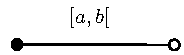
\includegraphics{figs/1/fig1.pdf}
  \end{figure}
  La longitud del segmento es 
  $$b-a=\text{longitud}([a,b[)=\l([a,b[).$$
  Si tenemos intervalos disjuntos
  \begin{figure}
    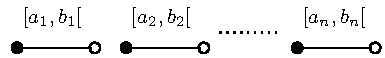
\includegraphics{figs/2/fig2.pdf}
  \end{figure}
  Entonces su longitud es $\sum_{i=1}^nb_i-a_i$.
\end{frame}

\begin{frame}{¿Cuál es la Longitud de un Punto?}
  Si tenemos $\set{a}\subseteq[a,a+\eps[$, entonces 
  $$\l(a)\leq \eps$$
  para $\eps>0$. De manera que la longitud del punto es cero.
\end{frame}

\begin{frame}{Los Racionales}
  Sea $\bQ\cap[0,1]=\set{q_n}\sucn$, entonces
  $$\l\left(\bigcup_{i=1}^n\set{q_i}\right)=\sum_{i=1}^n\l(\set{q_i})=0.$$
  Entonces, ¿cuál es la longitud de $\bQ\cap[0,1]$? Note que $\displaystyle\int_a^b\dd x=b-a$. 
\end{frame}

\begin{frame}{Unas Observaciones}
  De hecho si $[a,b[\subseteq[0,1]$, entonces
  \begin{enumerate}[(i)]
    \item $\displaystyle b-a=\int\limits_0^1\ind_{\lbonj{a,b}}(x)\dd x$.
    \item $\displaystyle \sum_{i=1}^nb_i-a_i=\int\limits_0^1\sum_{i=1}^n\ind_{\lbonj{a_i,b_i}}(x)\dd x=\int\limits_0^1\ind_{\bigcup_{i=1}^n\lbonj{a_i,b_i}}(x)\dd x$.
    \item $\displaystyle 0=\int\limits_0^1\ind_{\set{a}}(x)\dd x$.
  \end{enumerate}
\end{frame}

\begin{frame}{Volviendo a la Pregunta}
  En este caso $\displaystyle\int\limits_0^1\ind_{\bigcup_{i=1}^n\set{q_i}}(x)\dd x=0$. Note que $\ind_{\lbonj{0,1}\cap\bQ}=\lim_{n\to\infty}\ind_{\bigcup_{i=1}^n\set{q_i}}$.\par 
  Luego si $\ind_{\lbonj{0,1}\cap\bQ}$ fuese integrable y se pudieren tomar límites, tenemos que 
  $$\int\limits_0^1\ind_{\bQ\cap\bonj{0,1}}(x)\dd x=\lim_{n\to\infty}\int\limits_0^1\ind_{\bigcup_{i=1}^n\set{q_i}}(x)\dd x=0.$$
  ¿Qué integral estamos usando? Recordemos que $\ind_{\bQ\cap\bonj{0,1}}$ no es Riemann integrable.
\end{frame}

\section{Definición de Medida Exterior}

\begin{frame}
  Consideremos las familias
  \begin{itemize}
    \item $\displaystyle S=\set{\lbonj{a,b}:\ a<b}\cup\set{\rbonj{-\infty,b}:\ b\in\bR}\cup\set{\lbonj{a,\infty}:\ a\in\bR}\cup \emptyset$.
    \item $\displaystyle\cS_1=\Set{\bigcup_{i=1}^n I_i;\ I_i\in S,\ 1\leq i\leq n}$.
  \end{itemize}
Note que $[a,b]\not\in\cS_1$, pero $\bR=\lbonj{-\infty,b}\cup\rbonj{b,\infty}\in\cS_1$. Por lo tanto, dado $A\subseteq\bR$, existe $B\in\cS_1$ tal que $A\subseteq B$.
\end{frame}

\begin{frame}{La Definición}\label{fr:unaPrimeraDefn}
  Definimos $m:\cS_1\to\bR$ por:
  \begin{enumerate}
    \item $m(\bonj{a,b})=b-a$ si $a<b$.
    \item $m(\lbonj{a,\infty})=m(\rbonj{-\infty,b})=\infty$.
    \item $m\left(\bigcup_{i=1}^k I_i\right)=\sum_{i=1}^kb_i-a_i$ para $I_i=[a_i,b_i]$ que satisface $\obonj{a_i,b_i}\cap\obonj{a_j,b_j}=\emptyset$ si $i\neq j$.
  \end{enumerate}
\end{frame}

\begin{frame}{¿Está bien definida?}
  
\end{frame}
\section*{Resumen}

\subsection*{Qu\'e vimos hoy}

\begin{frame}{Resumen}

  % Keep the summary *very short*.
  \begin{itemize}
  \item Una definición de longitud de intervalo que nos lleva a preguntas nuevas.
  \item La primera definición de medida \ref{fr:unaPrimeraDefn}.
  \end{itemize}
  
\end{frame}

\subsection*{Ejercicios a trabajar}
\begin{frame}{Ejercicios}
    
  \begin{itemize}
    \item
      Lista 12
      \begin{itemize}
      \item 
      \end{itemize}
    \end{itemize}
  
\end{frame}


% All of the following is optional and typically not needed. 
\appendix
\section<presentation>*{\appendixname}
\subsection<presentation>*{Lectura adicional}

\begin{frame}[allowframebreaks]
  \frametitle<presentation>{Lecturas adicionales}
    
  \begin{thebibliography}{10}
    
  \beamertemplatebookbibitems
  % Start with overview books.

  \bibitem{CambroNotas}
    S.Cambronero.
    \newblock {\em Notas MA0505}.
    \newblock 20XX.

    \bibitem{NachoNotas}
    I.Rojas
    \newblock {\em Notas MA0505}.
    \newblock 2018.
 
  \end{thebibliography}
  
\end{frame}
%% 6 - 2:10:52 48
%% 7 - 1:17:44 44
%% 8 - 27:37 69
%% 9 - 1:07:47 86 + 59:38 40 approx 2 h c 7 min
%% 10 - 2:22:39 63
\end{document}


